\section{Atomic Structure}
Electrons, and all matter, behave like waves, which can undergo constructive and destructive
interference.

\begin{tabularx}{\linewidth}{|l|X|l|} \hline
    \multicolumn{3}{|c|}{$\lambda = \frac{h}{mv}$} \\ \hline
    & \textbf{value} & \textbf{unit} \\ \hline
    $\lambda$ & De Broglie wavelength & m \\ \hdashline
    $h$ & Planck's constant $= 6.626 \times 10^{-34}$& J/s \\
    $m$ & particle mass & \si{\kilo\gram} \\
    $v$ & particle velocity & \si{\metre\per\sec}\\ \hline
\end{tabularx}

By \textbf{Heisenberg's uncertainty principle}, it is impossible to know the precise position
of electrons in an atom.

\subsection{Quantum Mechanical Model}
A \textbf{wave equation} describes the behavior of a specific electron in an atom.

The solution to the wave equation is called a \textbf{wave function} ($\psi$), 
or an \textbf{orbital} --- the space boundary where there is a 95\% chance of finding the electron.

$|\psi|^2$ is proportional to the \emph{probability density} of an electron being found in 3D space.

The position of an electron could be described using \textit{Cartesian coordinates}, using the wave
equation $\psi(x, y, z)$.

Alternatively, using \textit{spherical coordinates}, $\psi(r, \theta, \phi)$:

\begin{tabularx}{\linewidth}{|l|X|l|} \hline
    \multicolumn{3}{|c|}{$\psi(r, \theta, \phi) = \mathbf{R}(r) \times \mathbf{Y}(\theta, \phi)$} \\ \hline
    & \textbf{value} & \textbf{unit} \\ \hline
    $\mathbf{R}(r)$ & \textbf{radial wave function} & -- \\
    $r$ & distance of the electron from the nucleus & -- \\ \hdashline
    $\mathbf{Y}(\theta, \phi)$ & \textbf{angular wave function} & -- \\
    $\theta$ & vertical angle perpendicular to the $x$-$y$ plane & -- \\
    $\phi$ & angle on the $x$-$y$ plane & -- \\ \hline
\end{tabularx}

\textbf{Radial nodes} are regions where the \textit{radial} component of the wave function passes through 0
--- appearing as a \emph{nodal sphere} expanding from the center, where no electrons are found.

\textbf{Angular nodes} are regions where the \textit{angular} component of the wave function passes through 0
--- appearing in the \emph{x-y plane} where no electrons are found.

In orbital diagrams, the regions corresponding to positive values of the wave function are shaded,
while the regions corresponding to negative values are not.

\subsubsection{Radial Distribution Function (RDF)}
\begin{tabularx}{\linewidth}{|l|X|l|} \hline
    \multicolumn{3}{|c|}{$RDF: 4 \pi r^2 \cdot \mathbf{R}(r)^2$ } \\ \hline
    & \textbf{value} & \textbf{unit} \\ \hline
    $4 \pi r^2$ & surface area of a sphere & -- \\
    $\mathbf{R}(r)$ & radial wave function & -- \\ \hline
\end{tabularx}

\vspace*{1em}
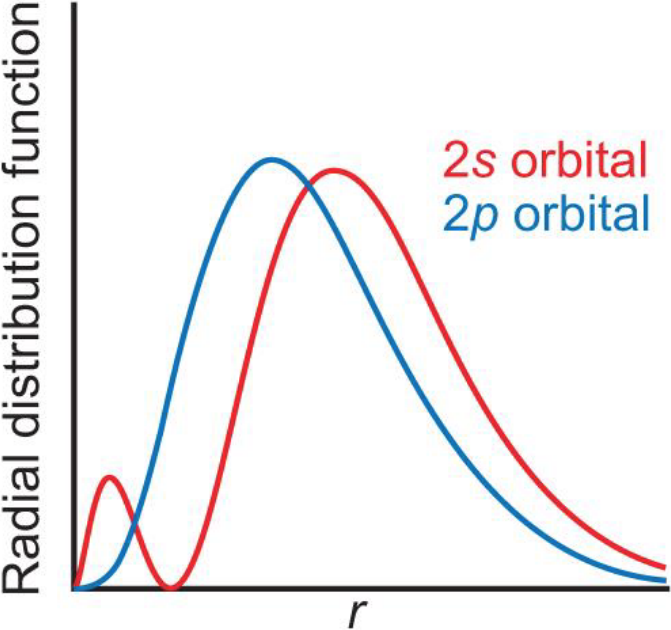
\includegraphics[width=\linewidth/2]{rdf}

The maximum value of the RDF (i.e. the peak) is the most probable distance of the electron
from the nucleus.

Even though the larger peak of the $2p$ orbital is closer than that of the $2s$ orbital,
the $2s$ orbital has a higher energy level than the $2p$ orbital due to the \textbf{penetration}
from the smaller peak.

Therefore, within shells of the same quantum number, orbital energy increases as follows:
 $s < p < d < f$.

 Radial nodes can be counted from the $x$-intercepts, so from the diagram above,
 the $2s$ orbital has 1 radial node, while the $2p$ orbital has none.

 \subsubsection{Quantum Numbers}
 \begin{tabularx}{\linewidth}{|l|X|X|} \hline
    \multicolumn{3}{|c|}{$nl_{m_l}$, e.g. $2p_z$} \\ \hline
    & \textbf{value} & \textbf{range} \\ \hline
    $n$ & \textbf{principal} QN & 1, 2, 3, \dots \\
    $l$ & \textbf{magnetic} QN & 1, \dots, $n-1$ \\
    $m_l$ & \textbf{orbital angular momentum} QN & $-l, \dots, 0, \dots, +l$ \\ \hline
\end{tabularx}

The principal QN relates to the \textit{size} and \textit{energy} of the orbital --- higher principal QNs
have larger orbitals with higher energy levels.

The magnetic QN relates to the \textit{shape} of the orbital.

The orbital angular momentum QN relates to the \textit{orientation} of the orbital.

\begin{tabularx}{\linewidth}{|Y|c|} \hline
    number of radial nodes & $l$ \\ \hline
    number of angular nodes & $n - l - 1$ \\ \hline
\end{tabularx}